\documentclass{article}
\usepackage[utf8]{inputenc}
\usepackage{enumitem}
\usepackage{amsmath}
\usepackage{titlesec}
\usepackage{graphicx}
\usepackage{float}
\restylefloat{figure}

\begin{document}

\title{Resumo P2}
\author{Patrick de Angeli}
\maketitle

\tableofcontents

\newpage

% \section{Plano de Negócios}

% \subsection{Definição}
% Um plano de negócios é um documento crucial para qualquer empreendimento, servindo como um guia detalhado que descreve os objetivos do negócio e os passos necessários para alcançá-los. Ele auxilia na identificação e mitigação de riscos e incertezas, aumentando as chances de sucesso do negócio.

% \subsection{Objetivos}
% \begin{itemize}
%     \item Testar a viabilidade da ideia, verificando se ela possui potencial de retorno econômico.
%     \item Orientar o desenvolvimento das operações e da estratégia, definindo o caminho a ser seguido pela empresa.
%     \item Atrair recursos financeiros, demonstrando a solidez do negócio para potenciais investidores.
%     \item Transmitir credibilidade para stakeholders, como bancos, investidores e parceiros.
%     \item Desenvolver a equipe de gestão, alinhando a visão e os objetivos do negócio a todos os membros da equipe.
% \end{itemize}

% \subsection{Estrutura}
% \begin{itemize}
%     \item \textbf{Sumário Executivo:} Apresentação concisa dos principais pontos do plano.
%     \item \textbf{Descrição da Empresa:} Detalhes sobre a empresa, como missão, visão, valores, estrutura organizacional, histórico e localização.
%     \item \textbf{Produtos e Serviços:} Descrição detalhada dos produtos e serviços oferecidos, incluindo seus diferenciais e vantagens competitivas. Análise do ciclo de vida do produto, considerar as diferentes etapas do ciclo de vida do produto (introdução, crescimento, maturidade e declínio) e como as estratégias de marketing e operações se adaptam a cada fase.
%     \item \textbf{Análise de Mercado:} Análise do mercado em que a empresa atua, incluindo a identificação do público-alvo, a análise da concorrência, as tendências de mercado e as oportunidades e ameaças.
%     \item \textbf{Plano de Marketing:} Estratégias para alcançar o mercado-alvo, incluindo as estratégias de produto, preço, praça (distribuição) e promoção.
%     \item \textbf{Plano Operacional:} Descrição detalhada de como a empresa irá operar, incluindo os processos de produção, a gestão de estoques, a logística e a infraestrutura.
%     \item \textbf{Plano Financeiro:} Projeções financeiras da empresa, incluindo as receitas, os custos, os investimentos, o fluxo de caixa e os indicadores de rentabilidade.
%     \item \textbf{Plano de Recursos Humanos:} Estratégias para a gestão de pessoas, incluindo o recrutamento, a seleção, o treinamento, o desenvolvimento, a remuneração e os benefícios.
%     \item \textbf{Análise de Riscos:} Identificação e análise dos principais riscos que a empresa enfrenta, bem como as estratégias para mitigá-los.
%     \item \textbf{Plano de Sustentabilidade:} Estratégias que visam garantir que a empresa tenha um impacto ambiental positivo ou neutro, incluindo o uso eficiente de recursos naturais, redução de emissões de carbono e responsabilidade social.
% \end{itemize}

% \subsection{Analise de Mercado}

% \begin{itemize}
%     \item \textbf{Análise da demanda:} Realizar uma previsão da demanda, considerando fatores como sazonalidade, tendências de mercado e comportamento do consumidor.
%     \item \textbf{Análise da concorrência:}  Incluir uma análise SWOT (Forças, Fraquezas, Oportunidades e Ameaças) dos principais concorrentes, identificando suas estratégias de marketing, preços e posicionamento.
%     \item \textbf{Pesquisa de marketing:} Descrever as fontes de dados (primárias e secundárias) que serão utilizadas para coletar informações sobre o mercado, clientes e concorrentes.
% \end{itemize}

\section{Marketing}

\subsection{Definição}
\textbf{Marketing} é o processo de criação, comunicação e entrega de valor para os clientes e para a gestão de relacionamentos com eles de forma que beneficiem a organização e seus stakeholders.

\begin{figure}[H]  % Use H para fixar a posição
    \centering
    \begin{minipage}{1.0\textwidth}
        \centering
        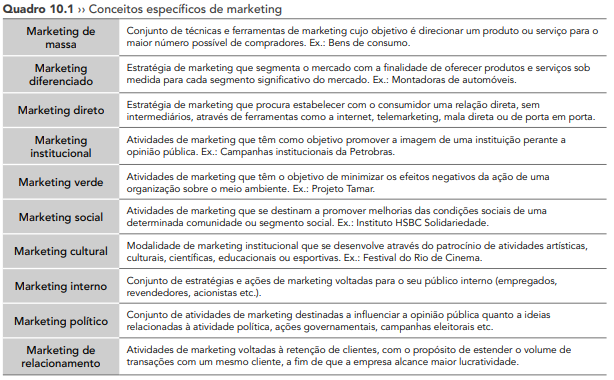
\includegraphics[width=\textwidth]{img/imagem10.png}
        \caption{Os tipos de marketing}  % Adicione uma legenda aqui
        \label{fig:exemplo}
    \end{minipage}
\end{figure}


\subsection{Processo de Marketing}
\begin{itemize}
    \item \textbf{Compreender o mercado e as necessidades dos clientes:} Através de pesquisa de mercado, o profissional de marketing precisa identificar as necessidades e desejos dos seus clientes, bem como as tendências e oportunidades do mercado.
    \item \textbf{Desenvolver uma estratégia de marketing orientada para o cliente:} Com base nas informações coletadas na etapa anterior, o profissional de marketing deve desenvolver uma estratégia de marketing que atenda às necessidades dos clientes e os posicione em relação à concorrência.
    \item \textbf{Construir um programa de marketing integrado que entregue valor superior:} O programa de marketing deve incluir um mix de marketing eficaz, que combine produto, preço, praça e promoção de forma sinérgica.
    \item \textbf{Construir relacionamentos lucrativos com os clientes:} O objetivo do marketing é construir relacionamentos duradouros com os clientes, que gerem valor para ambas as partes.
    \item \textbf{Capturar valor dos clientes para criar lucros e valor para o cliente:} O sucesso do marketing é medido pela capacidade da empresa de capturar valor dos clientes, gerando lucro e satisfação.
\end{itemize}

\subsection{Mix de Marketing}
\begin{itemize}
    \item \textbf{Produto:} Desenvolvimento e gestão de produtos que atendam às necessidades do mercado. 
    \begin{itemize}
        \item \textbf{Ciclo de Vida do Produto:} Introdução, crescimento, maturidade e declínio. 
    \end{itemize}
    \item \textbf{Preço:} Definição de estratégias de preço considerando custos, valor percebido e concorrência. 
    \item \textbf{Praça:} Distribuição dos produtos de forma a garantir sua disponibilidade para o consumidor. 
    \item \textbf{Promoção:} Comunicação com o mercado para divulgar o produto e persuadir a compra. 
    \begin{itemize}
        \item \textbf{Ferramentas de promoção:} Publicidade, propaganda, relações públicas, vendas pessoais e marketing digital. 
    \end{itemize}
\end{itemize}

\section{Operações}

\subsection{Definição}
\textbf{Administração de operações} é a área de administração que trata da gestão dos recursos e das atividades necessárias para a produção de bens e serviços.

\subsection{Fundamentos da Administração de Operações}
\begin{itemize}
    \item \textbf{Definição:} A administração de operações lida com a criação de bens e serviços, transformando insumos em produtos acabados. 
    \item \textbf{Tipos de organizações:} Manufatura (bens tangíveis) e serviços (bens intangíveis). 
    \item \textbf{Importância da administração de operações:} Impacto na produtividade, competitividade e lucratividade. 
    \item \textbf{Relação com outras áreas da administração:} Interconexão com marketing, finanças e recursos humanos. 
\end{itemize}

\subsection{Planejamento Estratégico do Sistema de Operações}
\begin{itemize}
    \item \textbf{Objetivo:} Projetar o sistema de operações para atender às necessidades estratégicas da organização. 
    \begin{enumerate}[label=\textbullet]
        \item \textbf{Planejamento e projeto do produto/serviço:} Define o que será produzido, características e qualidade.
        \item \textbf{Planejamento da capacidade:} Determina a quantidade a ser produzida, considerando a demanda e recursos.
        \item \textbf{Planejamento da localização:} Escolhe o local ideal para a produção, levando em conta custos, infraestrutura e mercado.
        \item \textbf{Planejamento do processo:} Define como a produção será organizada, incluindo tecnologia e arranjo físico.
        \item \textbf{Planejamento do layout:} Dispõe os recursos físicos de forma eficiente para otimizar o fluxo de trabalho.
    \end{enumerate}
\end{itemize}


\subsection{Processo de Transformação}

O processo de transformação é o núcleo da \textbf{Administração de Operações}, responsável por converter \textbf{insumos} em \textbf{produtos} ou \textbf{serviços}. Esse processo permeia toda a organização, impactando e sendo impactado por outras áreas funcionais. A visão sistêmica é crucial para a compreensão da administração de operações e do processo de transformação.

O processo de transformação pode ser compreendido em três etapas principais:

\textbf{1. Entrada (Input):}

Compreende os recursos que serão utilizados no processo de transformação. Eles podem ser classificados em duas categorias:

\begin{itemize}
\item \textbf{Recursos Transformados:} São os recursos que sofrem alterações durante o processo.
    \begin{itemize}
    \item Exemplos: Matérias-primas em uma fábrica, pacientes em um hospital, informações em um sistema contábil.
    \end{itemize}
\item \textbf{Recursos de Transformação:} São os recursos que atuam sobre os recursos transformados.
    \begin{itemize}
    \item Exemplos: Instalações, equipamentos, tecnologias, trabalhadores.
    \end{itemize}
\end{itemize}

\textbf{2. Processo de Transformação:}

É a etapa onde os insumos são convertidos em produtos ou serviços. Os tipos de processamento variam de acordo com a natureza do recurso transformado.

\begin{itemize}
\item \textbf{Processamento de Materiais:} Envolve a alteração das propriedades físicas dos materiais.
    \begin{itemize}
    \item Exemplos: Indústrias manufatureiras, empresas de transporte, empresas de armazenagem.
    \end{itemize}
\item \textbf{Processamento de Informações:} Envolve a modificação das características, posse, estocagem ou localização das informações.
    \begin{itemize}
    \item Exemplos: Empresas de contabilidade, institutos de pesquisa de mercado, bibliotecas, empresas de telecomunicações.
    \end{itemize}
\item \textbf{Processamento de Consumidores:} Envolve a alteração da localização, estado físico ou psicológico, ou acomodação dos consumidores.
    \begin{itemize}
    \item Exemplos: Empresas de turismo, hospitais, hotéis.
    \end{itemize}
\end{itemize}

\textbf{3. Saída (Output):}

Consiste nos bens ou serviços resultantes do processo de transformação. As características dos outputs variam de acordo com o tipo de processo e os insumos utilizados.

\begin{itemize}
\item \textbf{Tangibilidade:} Grau em que o output pode ser tocado.
\item \textbf{Estocabilidade:} Capacidade de armazenar o output.
\item \textbf{Transportabilidade:} Facilidade de transportar o output.
\item \textbf{Qualidade:} Grau de conformidade com as especificações e expectativas do cliente.
\end{itemize}

\section{Administração Financeira}

\subsection{A Administração Financeira nas Organizações}
\begin{itemize}
    \item \textbf{Definição:} Gestão dos recursos financeiros da organização, visando maximizar o valor da empresa. 
    \item \textbf{Objetivo da administração financeira:} Alocação eficiente de recursos, tomada de decisão de investimento e financiamento e geração de retorno para os acionistas. 
    \item \textbf{Funções do administrador financeiro:} Planejamento financeiro, análise de investimentos, gestão de capital de giro, captação de recursos e gestão de riscos. 
\end{itemize}

\subsection{Ciclos da Empresa}
\begin{itemize}
    \item \textbf{Ciclo de Investimento:} Aquisição de ativos para gerar receitas futuras. 
    \item \textbf{Ciclo de Financiamento:} Captação de recursos para financiar os investimentos. 
    \item \textbf{Ciclo de Exploração:} Operações diárias da empresa, desde a compra de insumos até a venda de produtos. 
\end{itemize}

\subsection{Sistema Financeiro}
\begin{itemize}
    \item \textbf{Instituições financeiras:} Intermediários financeiros que facilitam a alocação de recursos (bancos, corretoras, seguradoras). 
    \item \textbf{Mercados financeiros:} Ambiente onde ocorre a negociação de ativos financeiros (ações, títulos de dívida, moedas). 
    \item \textbf{Objetivo do sistema financeiro:} Canalizar recursos de agentes superavitários para agentes deficitários. 
\end{itemize}

\begin{figure}[H]  % Use H para fixar a posição
    \centering
    \begin{minipage}{1.0\textwidth}
        \centering
        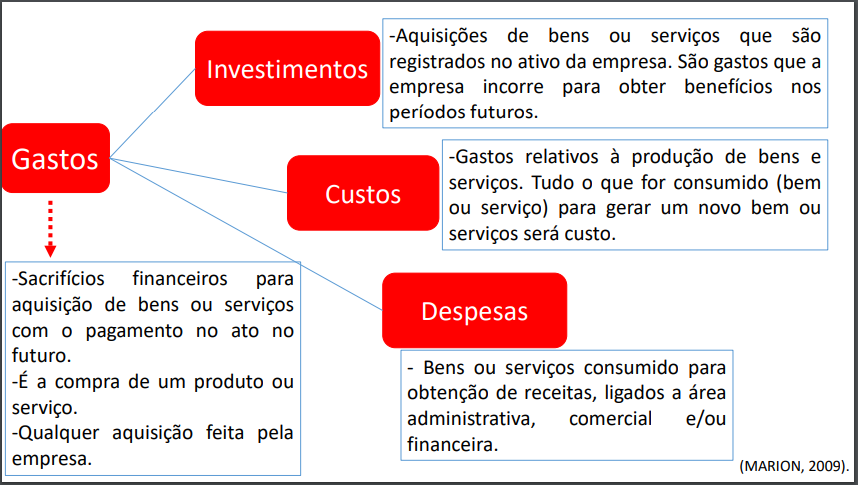
\includegraphics[width=\textwidth]{img/imagem9.png}
        \caption{Descrição da imagem}  % Adicione uma legenda aqui
        \label{fig:exemplo}
    \end{minipage}
\end{figure}


\subsection{Demonstrações Financeiras}
\begin{itemize}
    \item \textbf{Balanço Patrimonial:} Apresenta a posição financeira da empresa em um determinado momento. 
    \begin{itemize}
        \item \textbf{Ativo:} Bens e direitos da empresa. 
        \item \textbf{Passivo:} Obrigações da empresa. 
        \item \textbf{Patrimônio Líquido:} Recursos próprios da empresa. 
    \end{itemize}
    \item \textbf{Demonstração de Resultados do Exercício (DRE):} Apresenta o resultado (lucro ou prejuízo) da empresa em um período. 
    \begin{itemize}
        \item \textbf{Receitas:} Valores recebidos pela venda de produtos ou serviços. 
        \item \textbf{Despesas:} Custos e gastos para gerar as receitas. 
    \end{itemize}
    \item \textbf{Demonstração de Fluxos de Caixa (DFC):} Apresenta a movimentação de caixa da empresa em um período. 
    \begin{itemize}
        \item \textbf{Atividades operacionais:} Fluxos de caixa relacionados às operações da empresa. 
        \item \textbf{Atividades de investimento:} Fluxos de caixa relacionados à aquisição e venda de ativos. 
        \item \textbf{Atividades de financiamento:} Fluxos de caixa relacionados à captação e amortização de dívidas. 
    \end{itemize}
\end{itemize}

\subsection{Decisões de Investimento}
\begin{itemize}
    \item \textbf{Investimento de capital:} Alocação de recursos em projetos de longo prazo. 
    \item \textbf{Processo de investimento de capital:} Geração de ideias, análise de viabilidade, seleção de projetos e acompanhamento e avaliação. 
    \item \textbf{Técnicas de análise de investimentos:} Valor Presente Líquido (VPL), Taxa Interna de Retorno (TIR) e Payback. 
\end{itemize}


\section{Administração de Recursos Humanos}

\subsection{A Administração de Recursos Humanos (ARH) nas Organizações}
\begin{itemize}
    \item \textbf{Definição:} Conjunto de práticas e políticas que gerenciam o fator humano nas organizações. 
    \item \textbf{Objetivo da ARH:} Atrair, desenvolver, manter e reter talentos. 
    \item \textbf{Importância da ARH:} Impacto na produtividade, clima organizacional e resultados da empresa. 
\end{itemize}

\subsection{Influências Ambientais na ARH}
\begin{itemize}
    \item \textbf{Fatores externos:} Globalização, mudanças tecnológicas, legislação trabalhista e mercado de trabalho. 
    \item \textbf{Fatores internos:} Estratégia organizacional, cultura e clima organizacional. 
\end{itemize}

\subsection{Atraindo Trabalhadores Competentes}
\begin{itemize}
    \item \textbf{Planejamento de RH:} Previsão das necessidades de mão de obra da organização. 
    \item \textbf{Recrutamento:} Processo de atração de candidatos para as vagas disponíveis. 
    \begin{itemize}
        \item \textbf{Fontes de recrutamento:} Internas e externas. 
    \end{itemize}
    \item \textbf{Seleção:} Escolha dos candidatos mais adequados às vagas. 
    \begin{itemize}
        \item \textbf{Técnicas de seleção:} Entrevistas, testes, dinâmicas de grupo e avaliação de currículos. 
    \end{itemize}
\end{itemize}


\end{document}